\documentclass[12pt]{report}
\usepackage{graphicx}
\usepackage[utf8]{inputenc}
\usepackage[spanish]{babel}
\usepackage{setspace}
\usepackage{geometry}
\usepackage{titlesec}
\usepackage{times}
\usepackage{mathptmx} % Use mathptmx instead of times
\usepackage{fancyhdr}
\usepackage{float}
\usepackage{tikz}
\usetikzlibrary{shapes.geometric, arrows}

\tikzstyle{startstop} = [rectangle, rounded corners, minimum width=3cm, minimum height=1cm,text centered, draw=black, fill=red!30]
\tikzstyle{io} = [trapezium, trapezium left angle=70, trapezium right angle=110, minimum width=3cm, minimum height=1cm, text centered, draw=black, fill=blue!30]
\tikzstyle{process} = [rectangle, minimum width=3cm, minimum height=1cm, text centered, draw=black, fill=orange!30]
\tikzstyle{decision} = [diamond, minimum width=3cm, minimum height=1cm, text centered, draw=black, fill=green!30]
\tikzstyle{arrow} = [thick,->,>=stealth]


% Configuración de márgenes
\geometry{
    top=2.5cm,
    left=3cm,
    right=3cm,
    bottom=2.5cm
}

% Configuración de interlineado
\onehalfspacing

% Configuración de títulos y subtítulos
\titleformat{\chapter}[display]
  {\normalfont\bfseries\centering}{}{0pt}{\fontsize{14}{16}\selectfont}
\titleformat{\section}
  {\normalfont\bfseries}{\thesection}{1em}{\fontsize{12}{14}\selectfont}
\titleformat{\subsection}
  {\normalfont\bfseries}{\thesubsection}{1em}{\fontsize{12}{14}\selectfont}


% Configuración de pie de página
  \fancyhf{}
\fancyfoot[R]{\thepage}
\pagestyle{fancy}
\fancypagestyle{plain}{
  \fancyhf{}
  \fancyfoot[R]{\thepage}
}

  \begin{document}
  \pagenumbering{roman}
%----- PORTADA ----
\setlength{\hoffset}{27 pt} % 1 (Para centrar más la portada)
\begin{titlepage}
{\centering
{\fontfamily{ptm}\scshape\bfseries\fontsize{29.16}{34.992}\selectfont Universidad de Guadalajara \par}
\vspace{0.5cm}
{\scshape\Large Centro Universitario de los Lagos \par}
\vspace{1cm}
{\scshape\Large División de Estudios de la Biodiversidad e innovación Tecnológica \par}
\vspace{1cm}
{\graphicspath{{imagenes/Portada}} %ruta de las imagenes

\includegraphics[width=0.3\textwidth]{image.png}\par}
\vspace{1cm}
% Título
{\scshape\large\bfseries Practica 6 \par}
\vspace{0.5cm}
% Materia
{\large \textbf{Asignatura:} \\Sistemas Embebidos\par}
\vfill
% Estudiante
{\large \textbf{Presenta:} \\Oscar Iván Moreno Gutiérrez \#220942754
\\Arnold Jonathan Bradley Mercado Plascencia \#220942835
\\Alejandro Orozco Ramirez \#217490257  \par}
\vfill
% Profesor
{\large \textbf{Profesor:} \\Dr. Afanador Delgado Samuel Mardoqueo \par}
\vfill
\vfill
% Fecha
\begin{flushright}
  {\normalsize \textbf {Fecha:} \\ \today}
\end{flushright}
\vfill}
{\large  \par}
\end{titlepage}
%----- FIN DE PORTADA ----

%----- ÍNDICE GENERAL ----
\tableofcontents
\newpage

%----- PALABRAS CLAVE ----
\pagenumbering{arabic}
\chapter*{Palabras Clave}
\addcontentsline{toc}{chapter}{Palabras Clave}
Aquí van las palabras clave de tu documento.
\newpage

%----- OBJETIVO ----
\chapter*{Objetivo}
\addcontentsline{toc}{chapter}{Objetivo}
Desarrollar coodigo de configuracion y ejecucion de los puertos GPIO de sistema embebido mediante lenguaje de alto nivel.

\newpage

%----- CONTENIDO ----
\chapter{Contenido}
\section{Material}
\begin{itemize}
    \item Raspberry Pi
    \item Protoboard
    \item Cables
    \item Resistencias
    \item 3 LEDs
    \item Push Button
\end{itemize}
\newpage
\section{Diagrama de Flujo del Programa}
\begin{tikzpicture}[node distance=1.2cm]
  % Define the blocks
\node (start) [startstop] {Start};
\node (init) [process, below of=start] {Initialize GPIO};
\node (setup) [process, below of=init] {Setup LED and Button Pins};
\node (loop) [decision, below of=setup, yshift=-1cm] {Button Pressed?};
\node (increment) [process, below of=loop, yshift=-1cm] {Increment Counter};
\node (check) [decision, below of=increment, yshift=-1cm] {Check Counter Value};
\node (led1) [process, below of=check, yshift=-1cm] {Turn On LED1};
\node (led2) [process, below of=led1, yshift=-1cm] {Turn On LED2};
\node (led3) [process, below of=led2, yshift=-1cm] {Turn On LED3, Turn Off LED1};
\node (offled2) [process, below of=led3, yshift=-1cm] {Turn Off LED2 and LED3};
\node (blink) [process, below of=offled2, yshift=-1cm] {Blink LED2};
\node (end) [startstop, below of=blink, yshift=-1cm] {End};

% Draw the arrows
\draw [arrow] (start) -- (init);
\draw [arrow] (init) -- (setup);
\draw [arrow] (setup) -- (loop);
\draw [arrow] (loop) -- node[anchor=east] {Yes} (increment);
\draw [arrow] (increment) -- (check);
\draw [arrow] (check) -- node[anchor=east] {Counter == 2} (led1);
\draw [arrow] (led1) -- (led2);
\draw [arrow] (led2) -- (led3);
\draw [arrow] (led3) -- (offled2);
\draw [arrow] (offled2) -- (blink);
\draw [arrow] (blink) -- (end);
\draw [arrow] (loop.east) -- ++(1,0) node[anchor=north] {No} |- (loop.west);

\end{tikzpicture}

\section{Programa en Python }
\begin{verbatim}
  import RPi.GPIO as GPIO
  import time
  ## Modo
  GPIO.setwarnings(False)
  GPIO.setmode(GPIO.BCM)

  ## Declaracion de Puertos
  buttonpin = 18
  led1,led2,led3 = 16,20,21

  ## Declaracion de direccion de puertos
  ## LEDS
  GPIO.setup(led1,GPIO.OUT)
  GPIO.setup(led2,GPIO.OUT)
  GPIO.setup(led3,GPIO.OUT)

  ## Boton
  GPIO.setup(buttonpin,GPIO.IN,pull_up_down=GPIO.PUD_UP)

  ##programa
  cont = 0
  res = False

  def prenderLED(ledID):
    GPIO.output(ledID,True)
  def apagarLED(ledID):
    GPIO.output(ledID,False)

  #def setPWM():

  try:
    while True:
      current_state = GPIO.input(buttonpin)
      if current_state == GPIO.LOW and not res:
        cont += 1
        print(f"Presion numero: {cont}")
        res = True
      if current_state == GPIO.HIGH:
        res = False

      ## PARTE DE PRENDER LEDS
      if cont == 2:
        prenderLED(led1)
      elif cont == 3:
        prenderLED(led2)
      elif cont == 4:
        prenderLED(led3)
        apagarLED(led1)
      elif cont == 5:
        apagarLED(led2)
        apagarLED(led3)
      elif cont == 6:
        time.sleep(1)
        prenderLED(led2)
        time.sleep(0.2)
        apagarLED(led2)

      elif cont == 7:
        print("FUgaaaaaa")
        break
      time.sleep(0.1)

  except KeyboardInterrupt:
    print("Adios")
  finally:
    GPIO.cleanup()
\end{verbatim}

\section{Codigo python con interrupciones}
\begin{verbatim}
  import RPi.GPIO as GPIO
  import time

  # Modo
  GPIO.setwarnings(False)
  GPIO.setmode(GPIO.BCM)

  # Declaracion de Puertos
  buttonpin = 4
  led1, led2, led3 = 16, 20, 21

  # Declaracion de direccion de puertos
  # LEDS
  GPIO.setup(led1, GPIO.OUT)
  GPIO.setup(led2, GPIO.OUT)
  GPIO.setup(led3, GPIO.OUT)

  # Boton
  GPIO.setup(buttonpin, GPIO.IN, pull_up_down=GPIO.PUD_UP)

  # Variables
  cont = 0
  res = False

  def prenderLED(ledID):
      GPIO.output(ledID, True)

  def apagarLED(ledID):
      GPIO.output(ledID, False)

  def button_callback(channel):
      global cont, res
      if not res:
          cont += 1
          print(f"Presion numero: {cont}")
          res = True

      # PARTE DE PRENDER LEDS
      if cont == 2:
          prenderLED(led1)
      elif cont == 3:
          prenderLED(led2)
      elif cont == 4:
          prenderLED(led3)
          apagarLED(led1)
      elif cont == 5:
          apagarLED(led2)
          apagarLED(led3)
      elif cont == 6:
          time.sleep(1)
          prenderLED(led2)
          time.sleep(0.2)
          apagarLED(led2)
      elif cont == 7:
          print("FUgaaaaaa")
          GPIO.cleanup()
          exit()

  # Setup interrupt
  GPIO.add_event_detect(buttonpin, GPIO.FALLING, callback=button_callback, bouncetime=200)

  try:
      while True:
          current_state = GPIO.input(buttonpin)
          if current_state == GPIO.HIGH:
              res = False
          time.sleep(0.1)

  except KeyboardInterrupt:
      print("Adios")
  finally:
      GPIO.cleanup()
\end{verbatim}
\section{Fotos}
\begin{figure}[H]
  \centering
  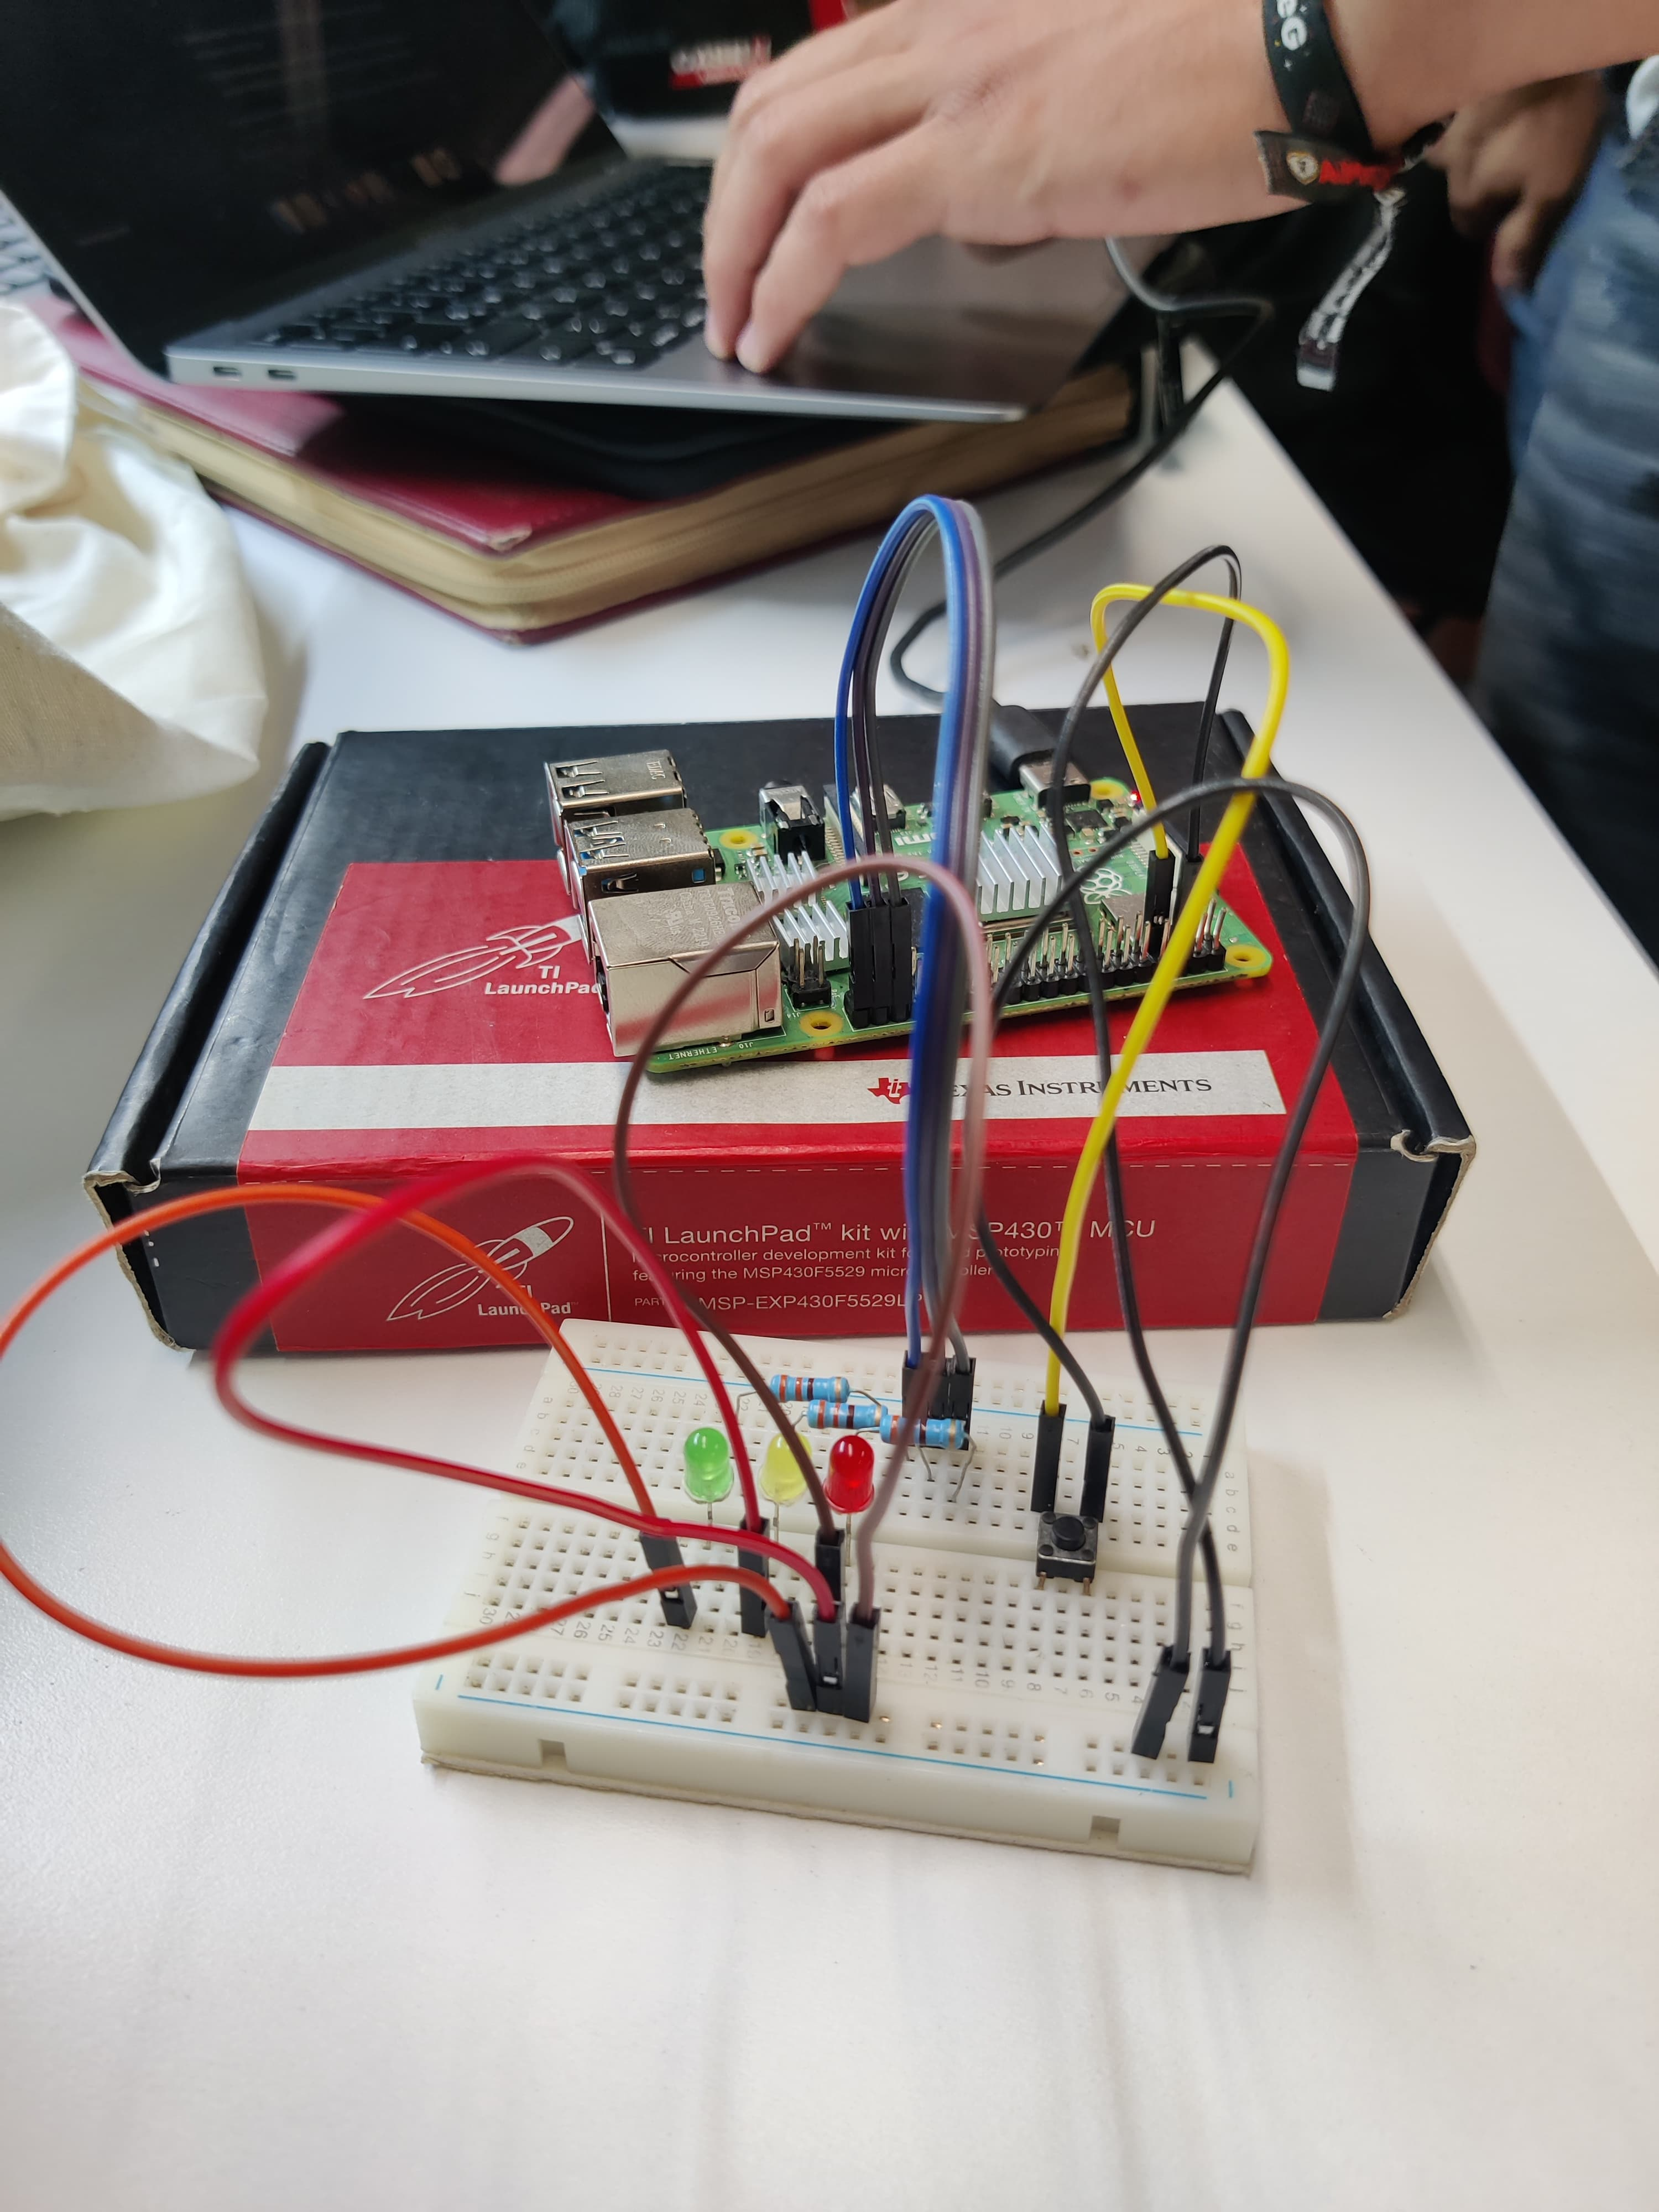
\includegraphics[width=0.5\textwidth]{screenshots/foto1.jpeg}
  \caption{En 0s}
\end{figure}
\begin{figure}[H]
  \centering
  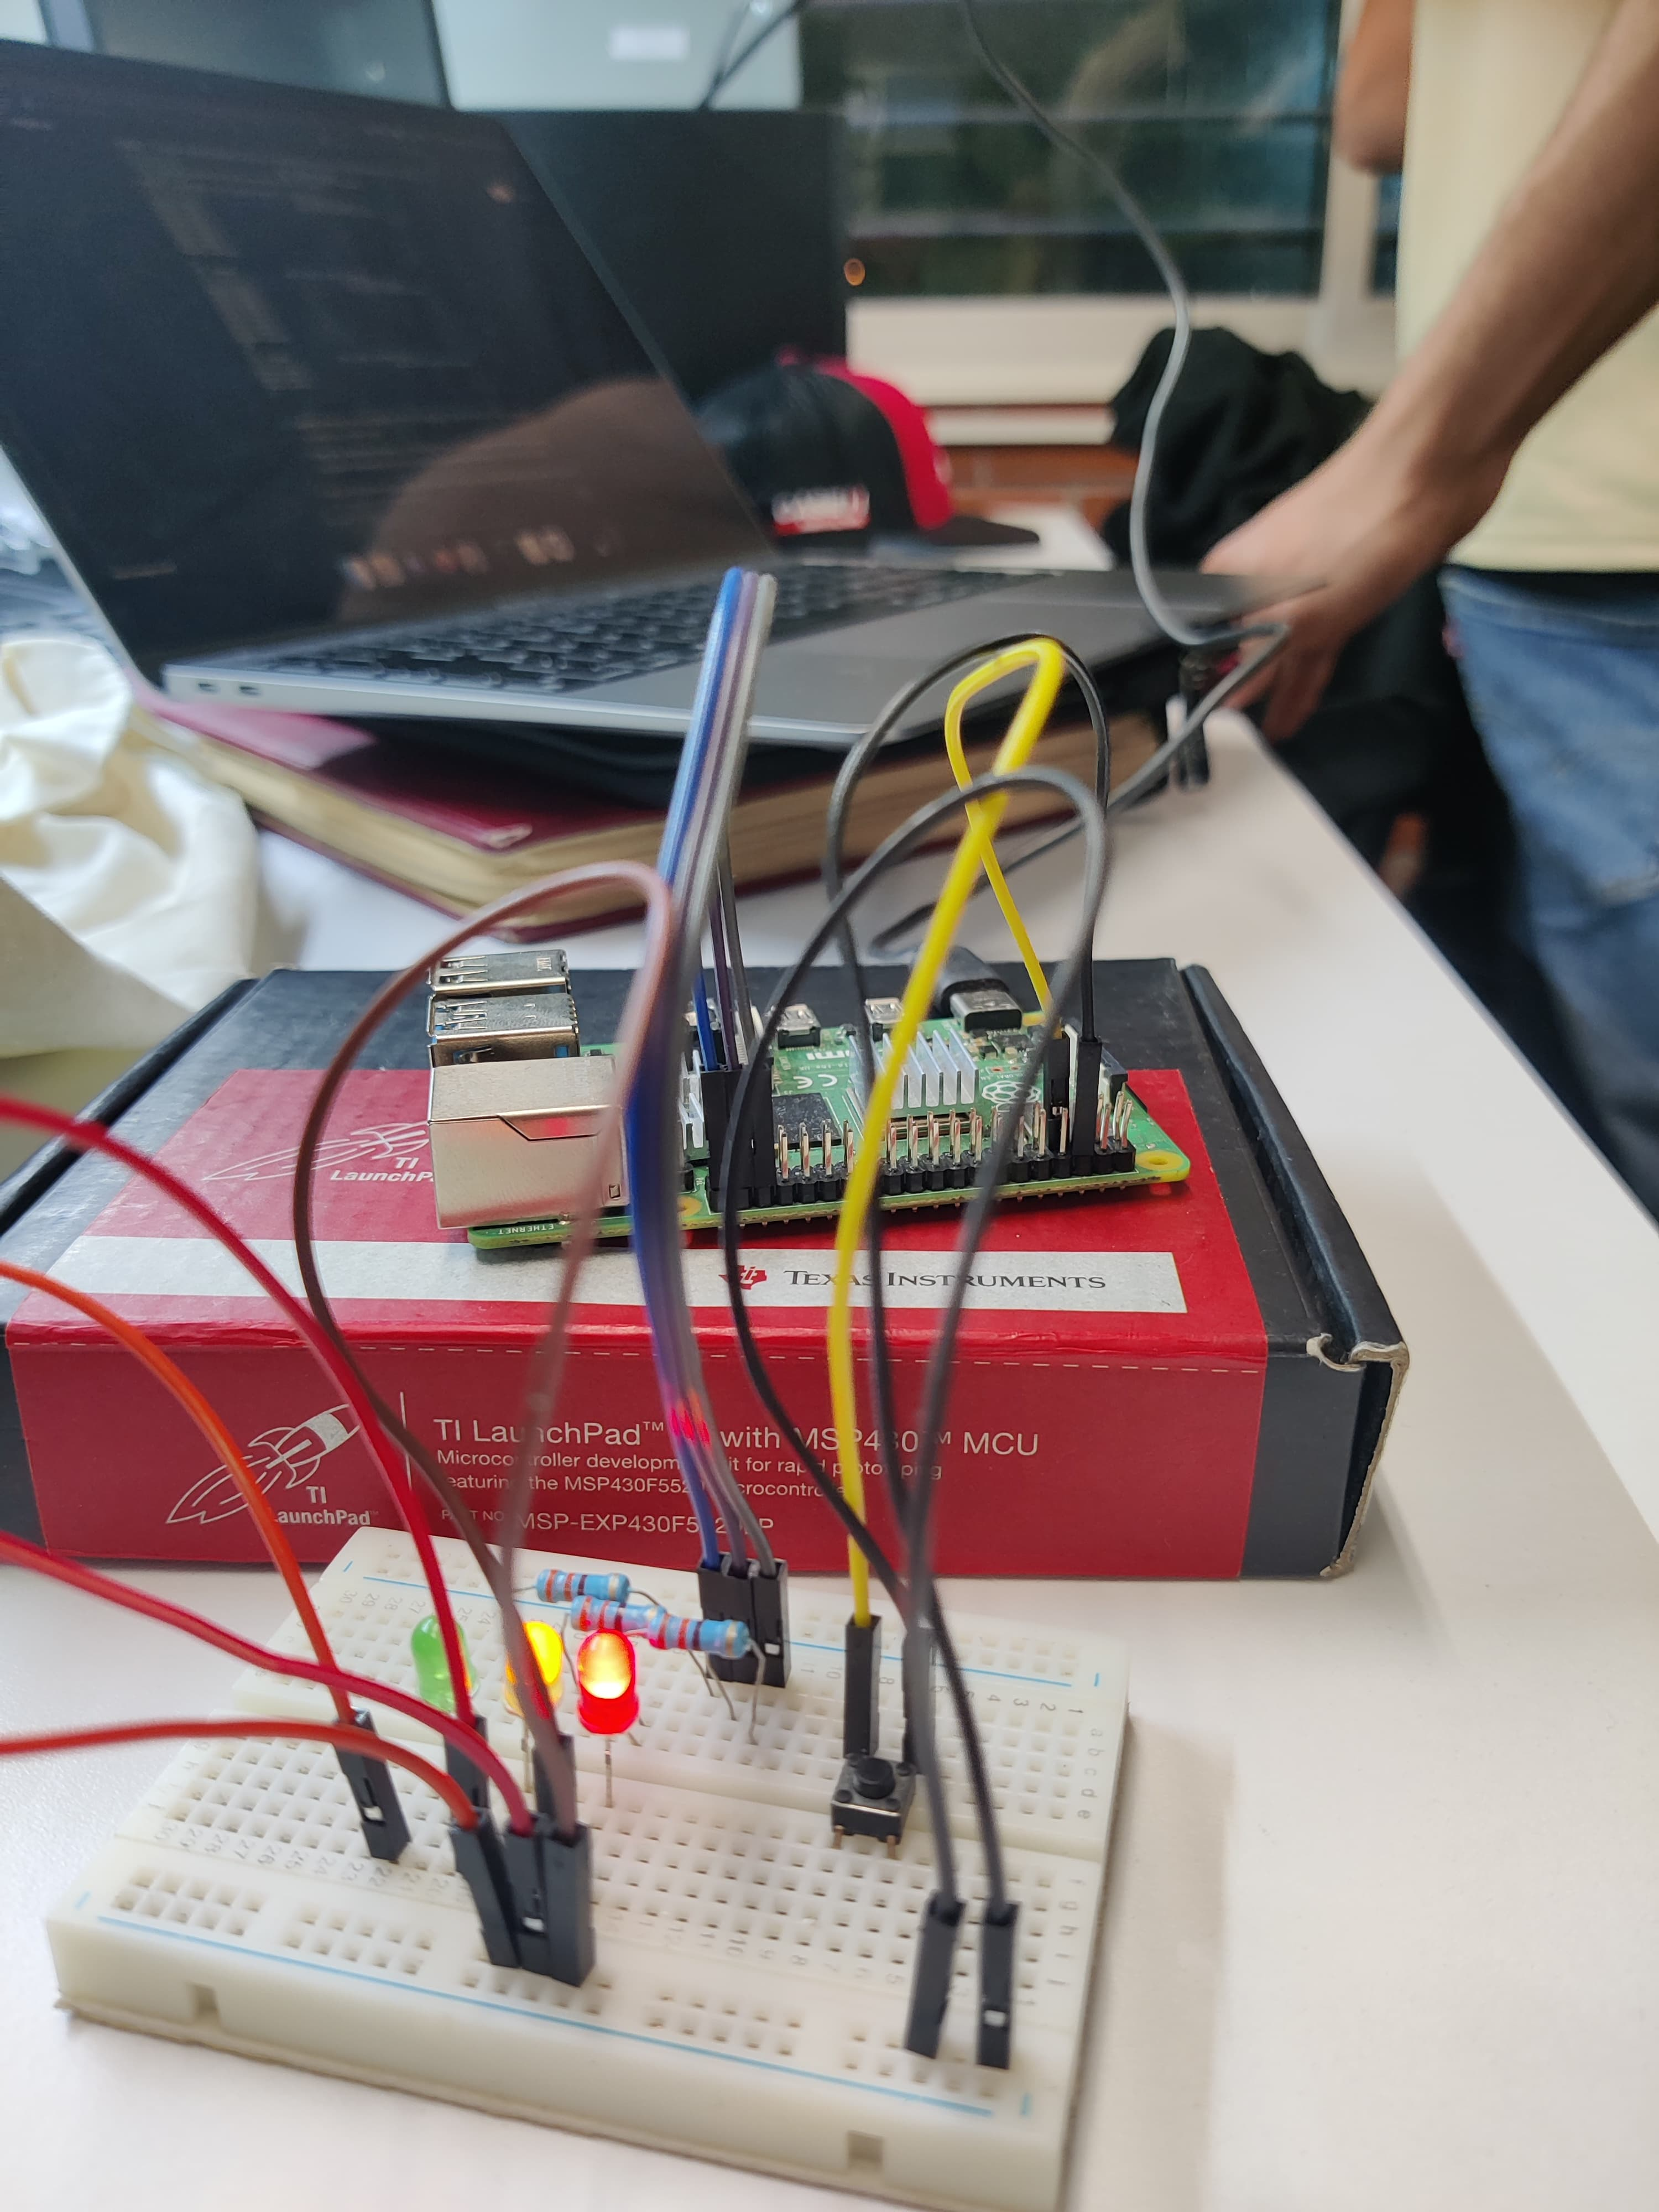
\includegraphics[width=0.5\textwidth]{screenshots/foto2.jpeg}
  \caption{3 pulsaciones}
\end{figure}
\begin{figure}[H]
  \centering
  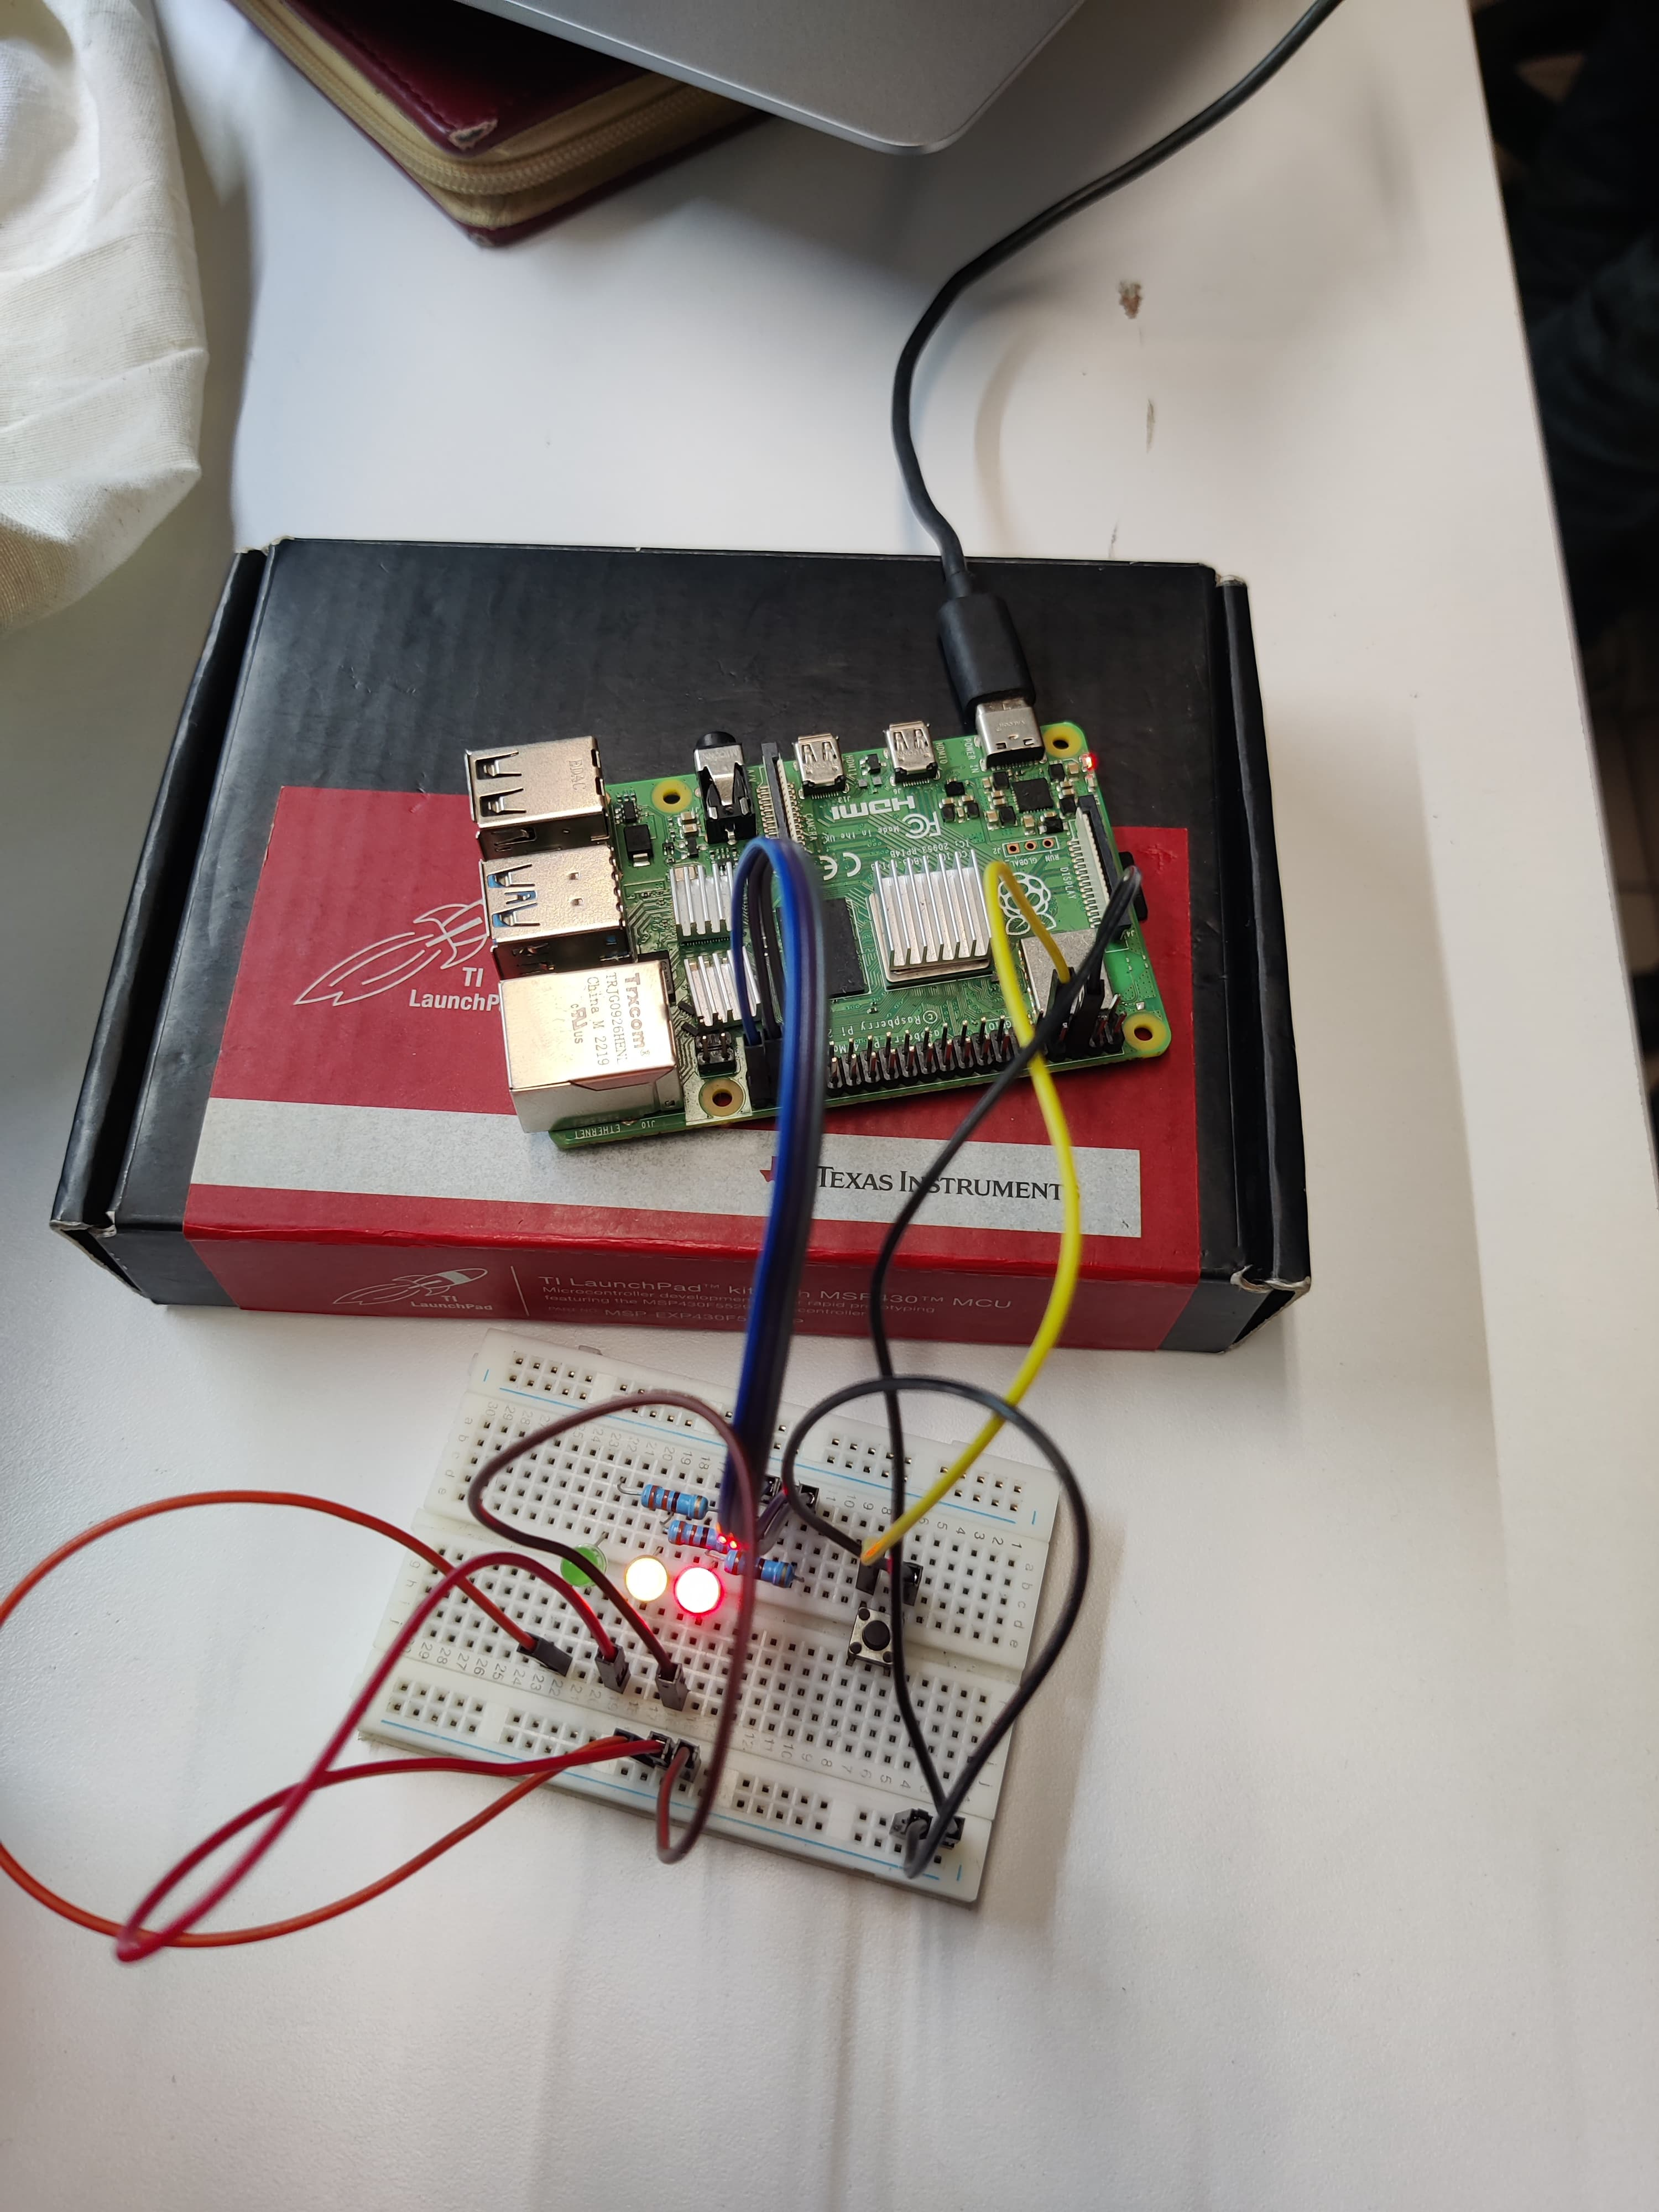
\includegraphics[width=0.5\textwidth]{screenshots/foto3.jpeg}
  \caption{3 pulsaciones tambien}
\end{figure}
\begin{figure}[H]
  \centering
  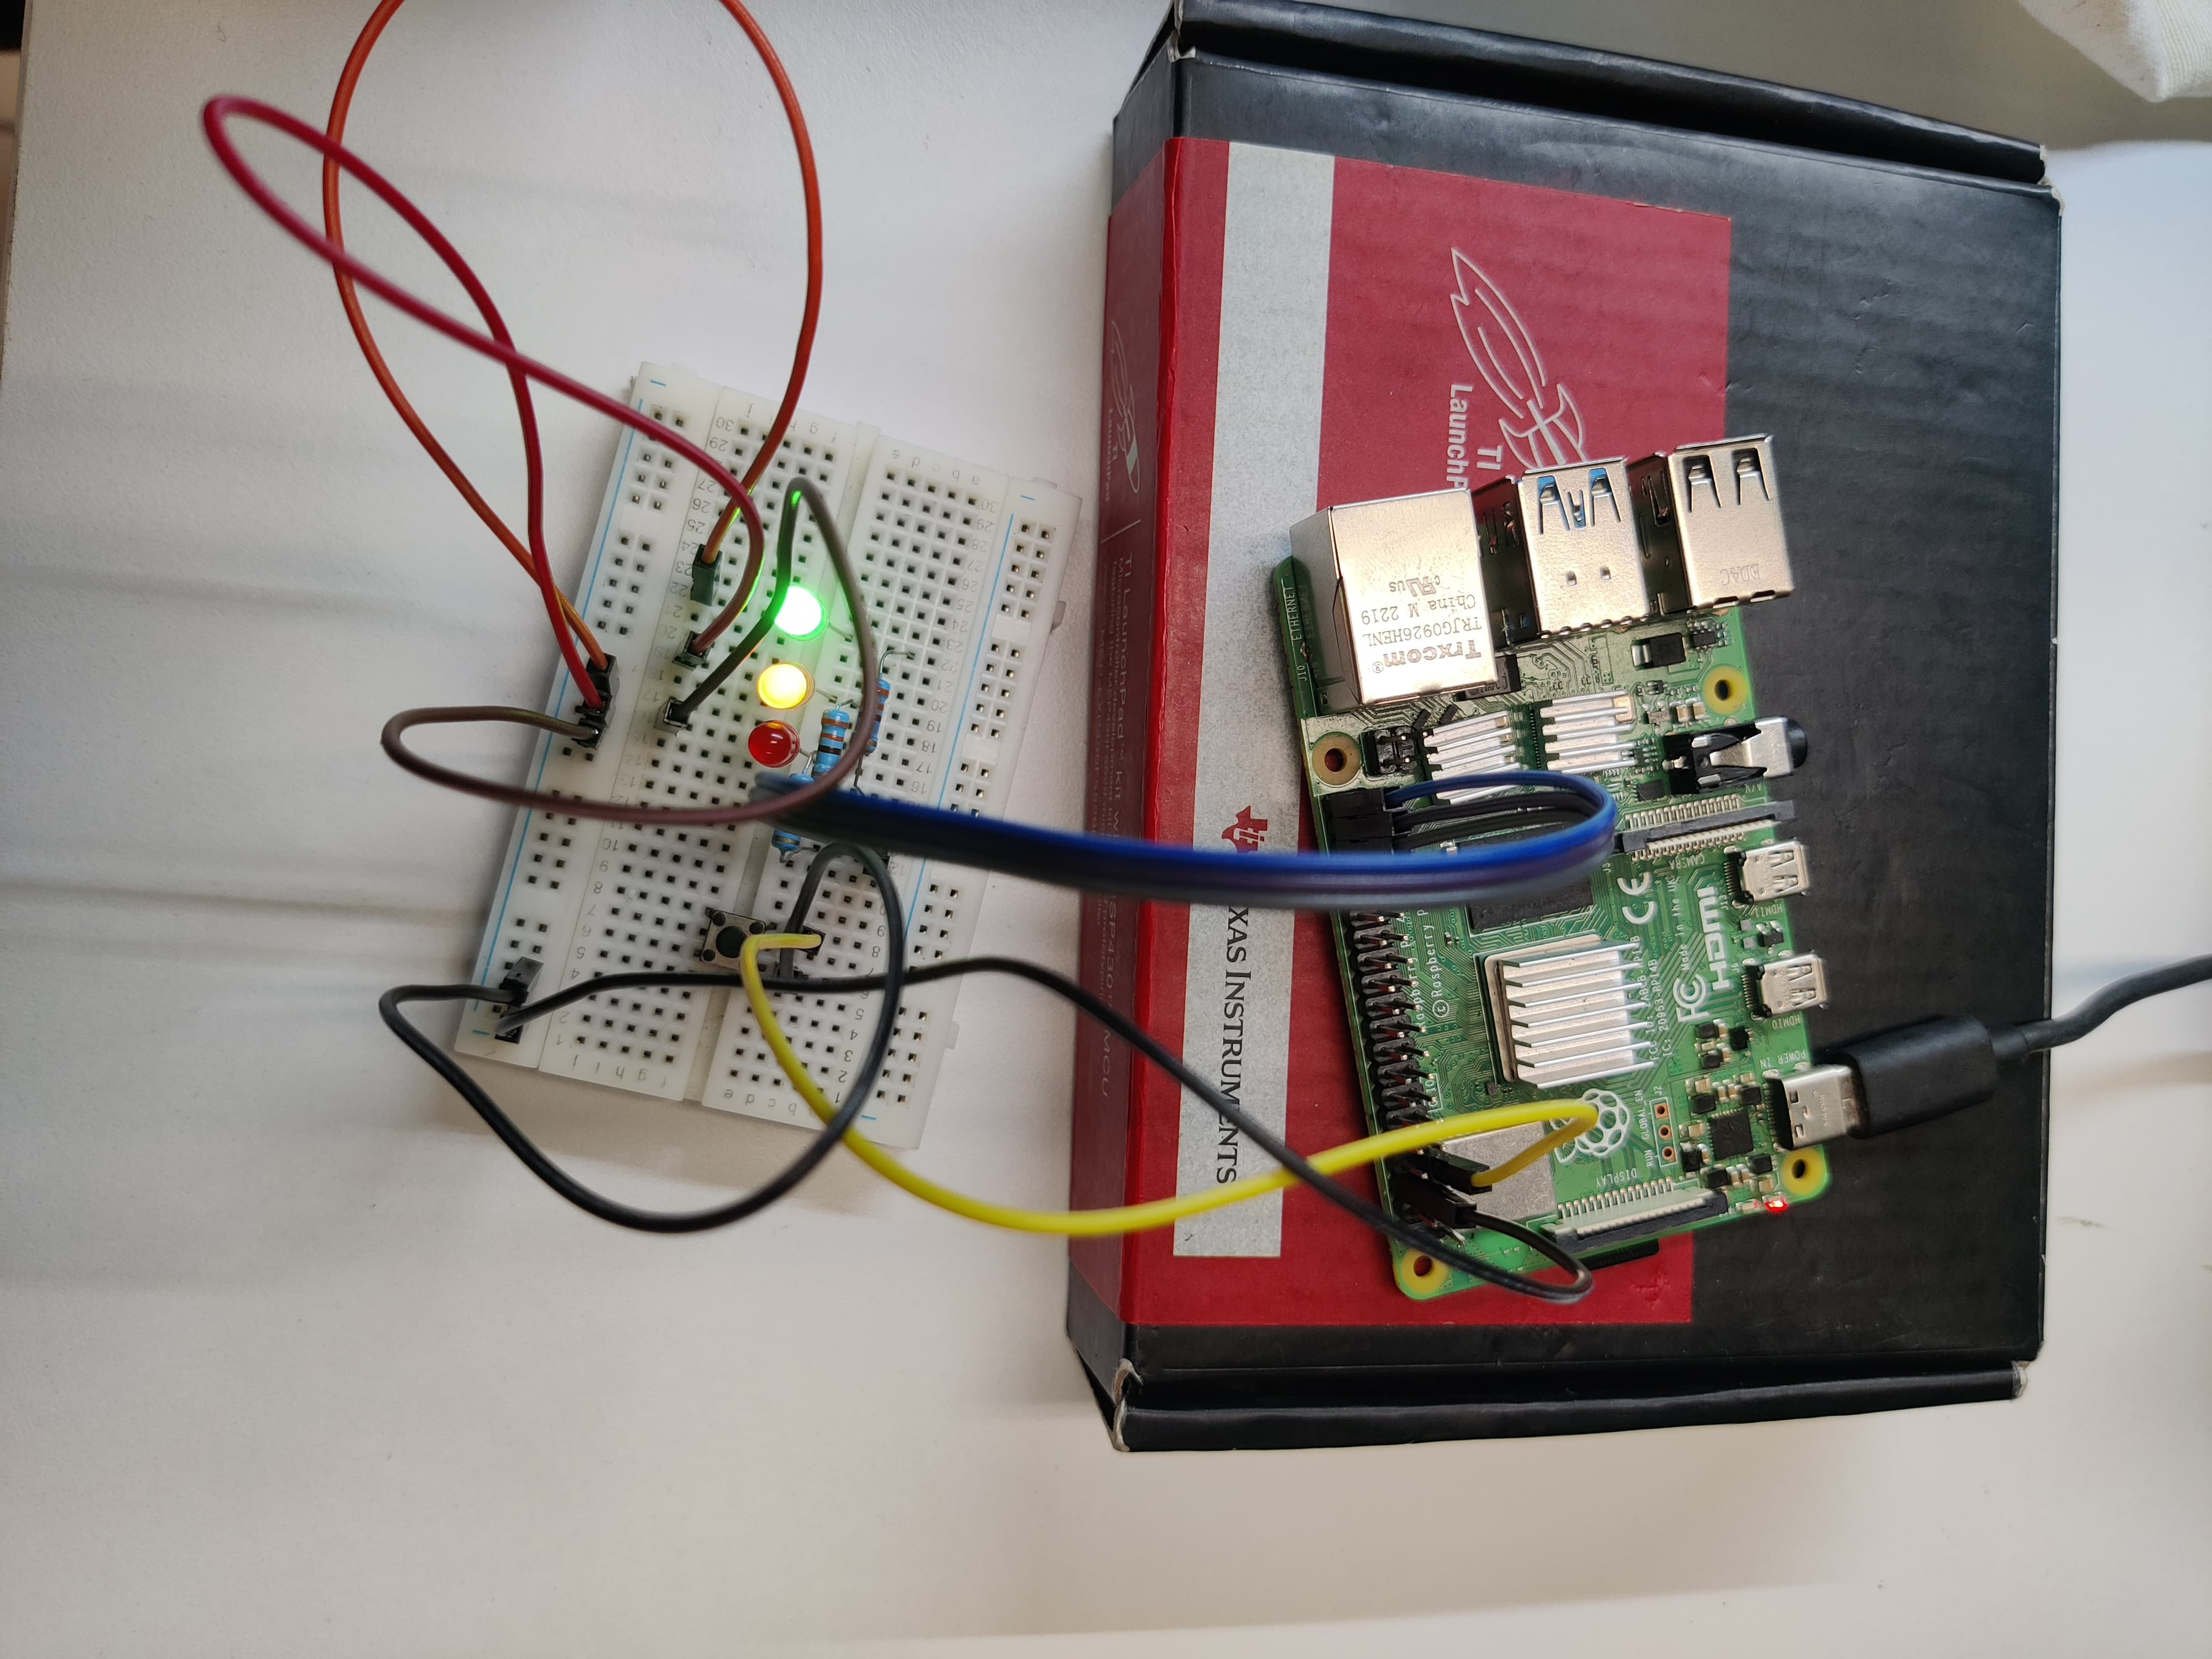
\includegraphics[width=0.5\textwidth]{screenshots/foto4.jpeg}
  \caption{4 pulsaciones}
\end{figure}
\newpage

%----- CONCLUSIONES ----
\chapter{Conclusiones}
Utilizando pollnig para hacer el program toma mas recursos del sistema, en cambio con interrupciones el sistema se mantiene en espera de una señal para ejecutar una accion, lo que hace que el sistema sea mas eficiente.
\newpage

%----- REFERENCIAS ----


\end{document}